% Appendix A
\chapter*{Appendix}
    \begin{table}[h]
        \centering
        \footnotesize
        \begin{tabular}{l|c}
        \toprule
        Metrics & Definition \\
        \midrule
        Cosine & $1 - \dfrac{f_t(u)\cdot f_t(v)}{\left||f_t(u)\right||_2\left||f_t(v)\right||_2}$ \\
        Euclidean & $\left||f_t(u) - f_t(v)\right||_2$ \\
        Correlation & $1-\dfrac{(f_t(u)-\overline{f_t(u)}) \cdot(f_t(v)-\overline{f_t(v)})}{||(f_t(u)-\overline{f_t(u)})||_{2}||(f_t(v)-\overline{f_t(v)})||_{2}}$ \\
        Chebyshev & $\max _{i}\left|f_{t_i}(u)-f_{t_i}(v)\right|$ \\
        Braycurtis & $\dfrac{\sum\left|f_{t_i}(u)-f_{t_i}(v)\right|} {\sum\left|f_{t_i}(u)+f_{t_i}(v)\right|}$ \\
        Manhattan & $\sum{i}\left|f_{t_i}(u)-f_{t_i}(v)\right|$ \\
        Canberra & $\sum_{i} \dfrac{\left|f_{t_i}(u)-f_{t_i}(v)\right|}{\left|f_{t_i}(u)\right|+\left|f_{t_i}(v)\right|}$ \\
        Sqeuclidean & $\left||f_t(u) - f_t(v)\right||_2^2$ \\
        \bottomrule
        \end{tabular}
        \caption{Distance metrics: $f_{t_i}(u)$ represents the $i$-th component of $f_t(u)$.}
        \label{table:distance}
    \end{table}

    \begin{table}[!h]
        \centering
        \footnotesize
        \begin{tabular}{l|l|}
          \toprule
          Notation & Description \\
          \midrule
          $f_t$ & Target GNN Model \\
          $D_{f_t}$ & Dataset used to train $f_t$ \\
          $A$ & Adversary \\
          $D_A$ & Dataset used to train $A$ \\
          $G_A$ & Graph used to sample $D_A$ \\
          $\alpha$ & Percentage of known edges in $G_A$ \\
          $G_A^{0.4}$ & Graph used to sample $D_A$ with 40\% known edges \\
          $f_A$ & GNN Model, that is involved in training $A$ \\
          $D_{f_A}$ & Dataset used to train $f_A$ \\
          $G_s$ & Incomplete Graph, $A$ performs link stealing attacks on \\
          \bottomrule
        \end{tabular}
        \caption{Notations}
        \label{table:notations}
      \end{table}

    \begin{figure}[h]
      \begin{center}
        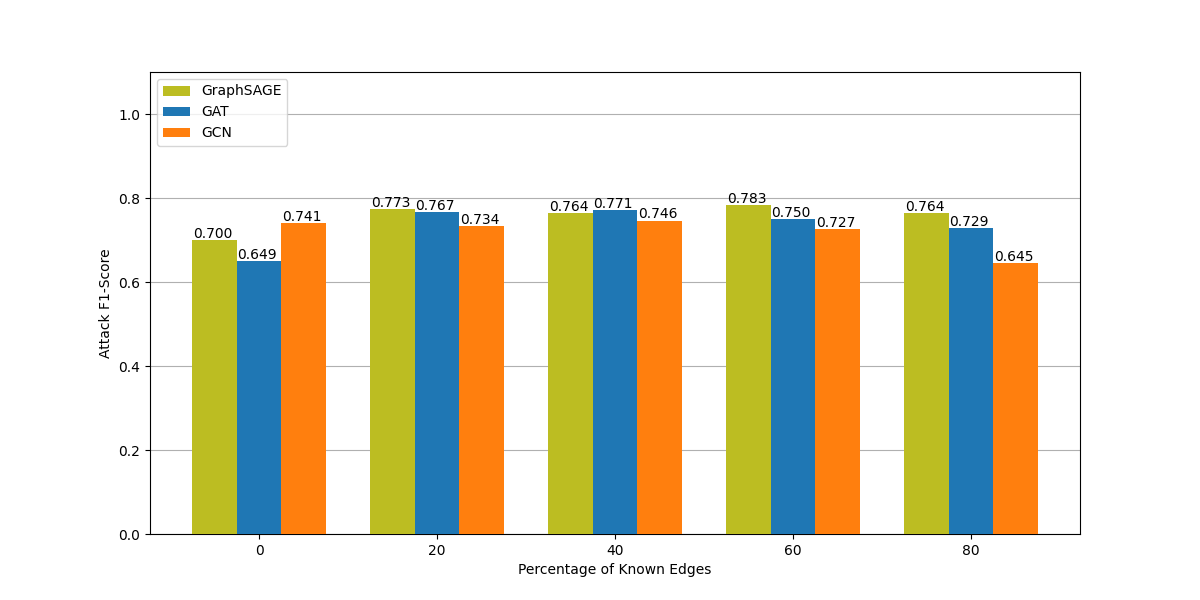
\includegraphics[width=\textwidth]{attack-1-cora}
        \caption{Attack 1 - $D_{f_t} = Cora$}
        \label{figure:eval-att1-cora}
      \end{center}
    \end{figure}

    \begin{figure}[h]
      \begin{center}
        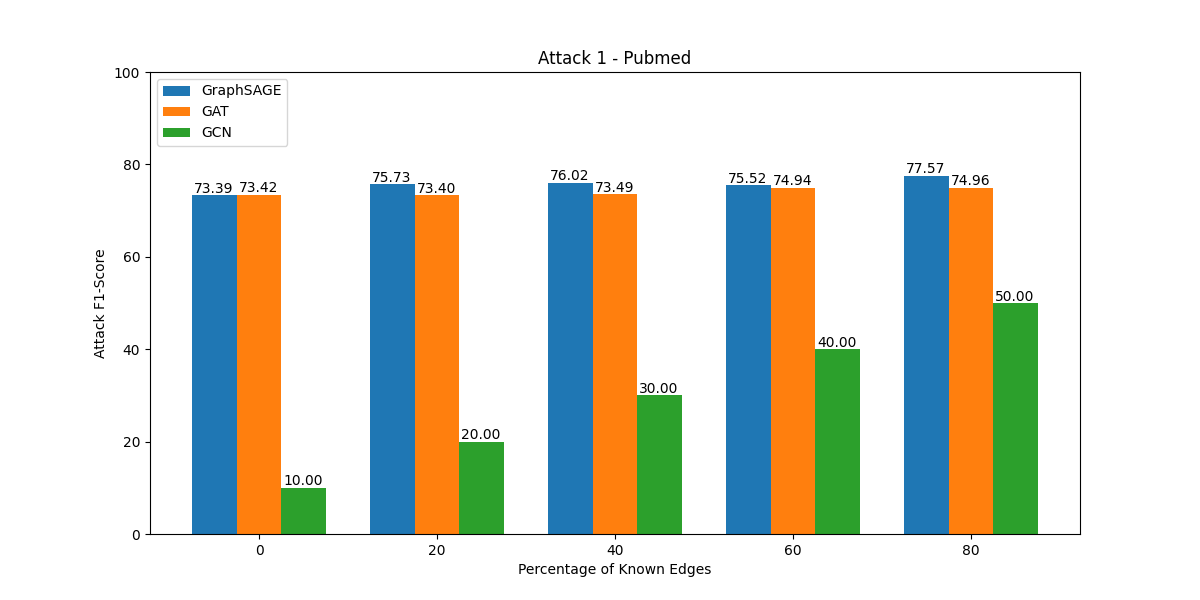
\includegraphics[width=\textwidth]{attack-1-pubmed}
        \caption{Attack 1 - $D_{f_t} = Pubmed$}
        \label{figure:eval-att1-pubmed}
      \end{center}
    \end{figure}

    \begin{figure}[h]
      \begin{center}
          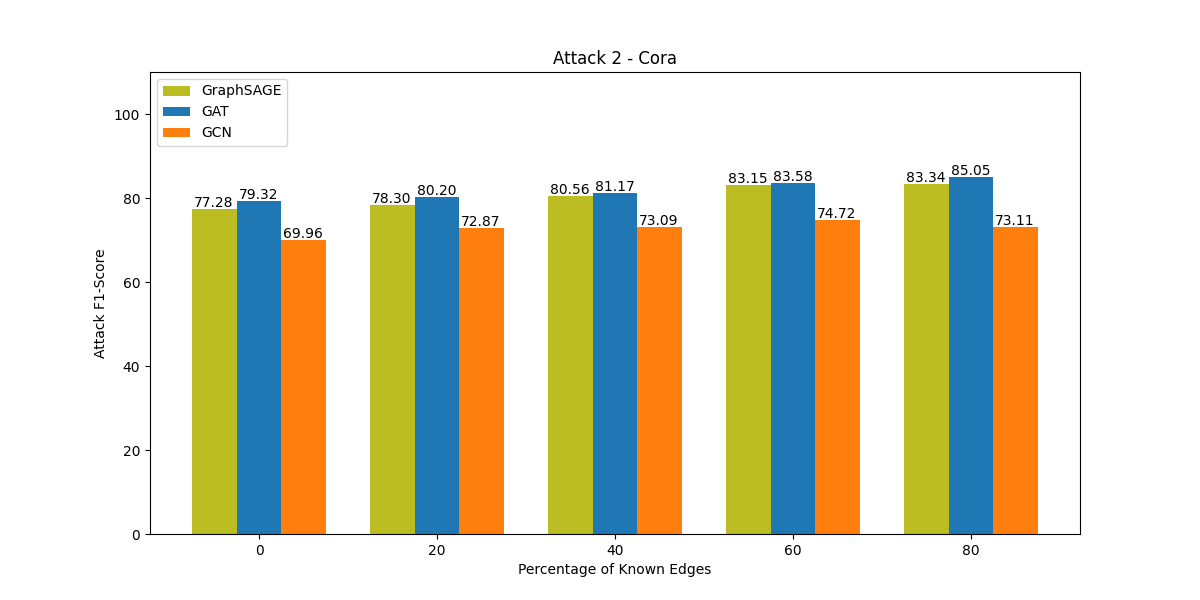
\includegraphics[width=\textwidth]{attack-2-cora}
          \caption{Attack 2 - $D_{f_t} = Cora$}
          \label{figure:eval-att2-cora}
      \end{center}
    \end{figure}

    \begin{figure}[h]
      \begin{center}
          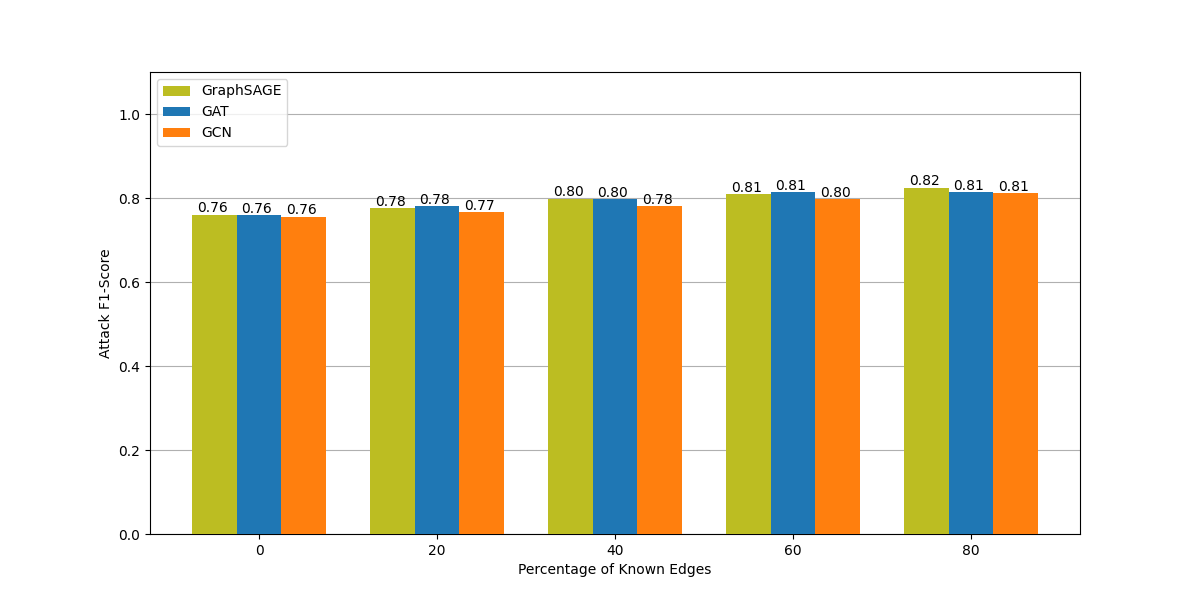
\includegraphics[width=\textwidth]{attack-2-pubmed}
          \caption{Attack 2 - $D_{f_t} = Pubmed$}
          \label{figure:eval-att2-pubmed}
      \end{center}
    \end{figure}

    \begin{figure}[h]
      \begin{center}
          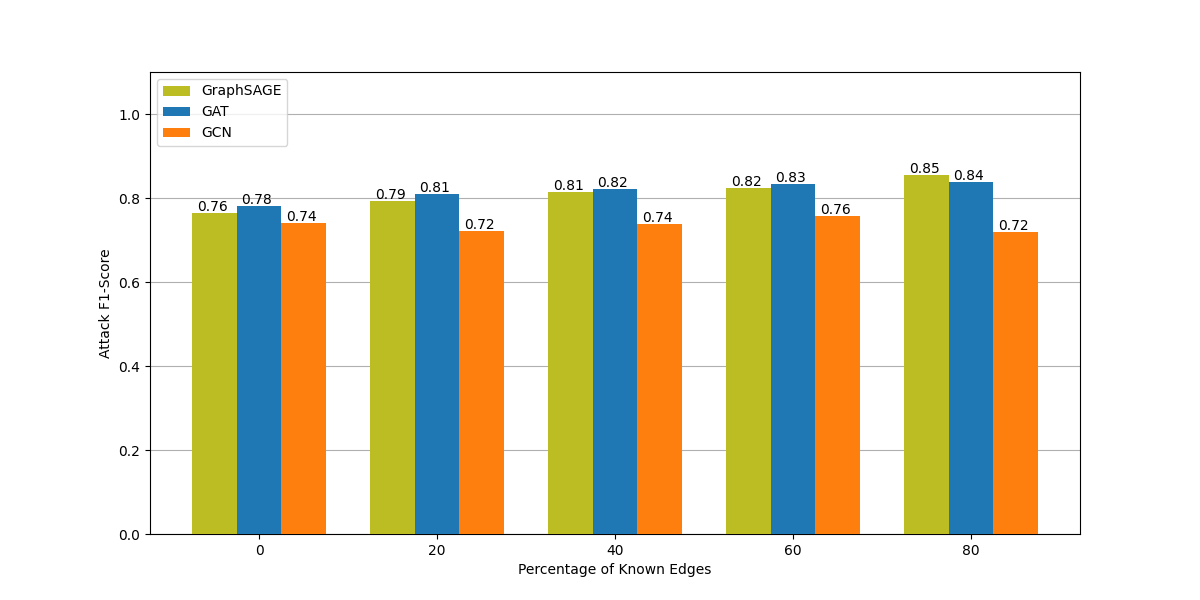
\includegraphics[width=\textwidth]{attack-3-citeseer-cora}
          \caption{Attack 3 - $D_{f_t} = Cora$ and $D_A = CiteSeer$}
          \label{figure:eval-att3-citeseer-cora}
      \end{center}
  \end{figure}

  \begin{figure}[h]
      \begin{center}
          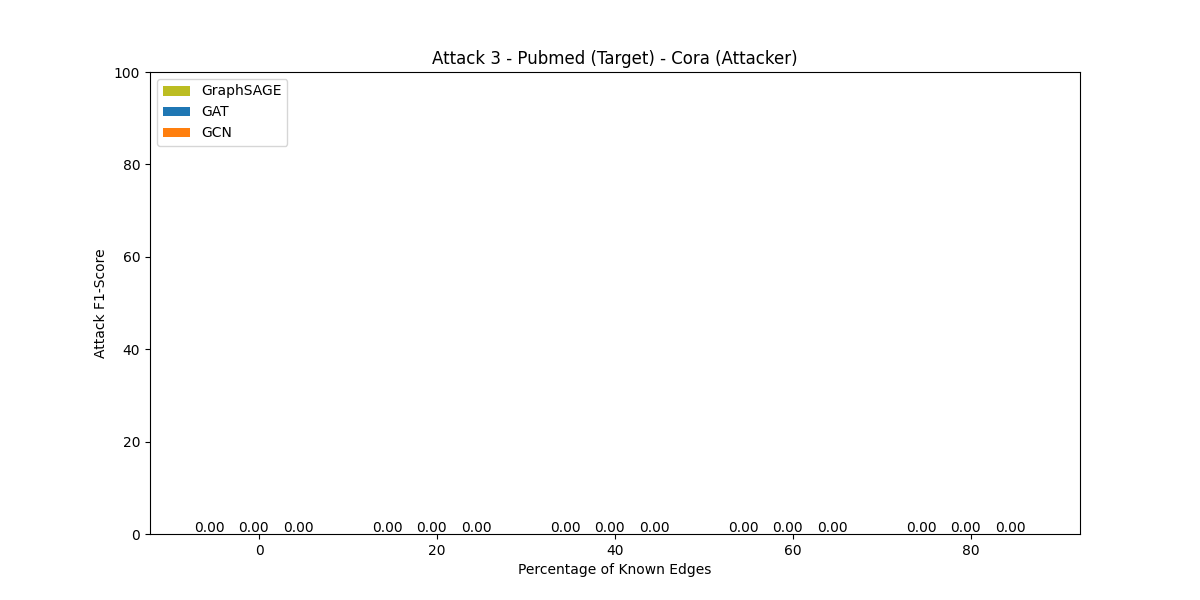
\includegraphics[width=\textwidth]{attack-3-pubmed-cora}
          \caption{Attack 3 - $D_{f_t} = Cora$ and $D_A = Pubmed$}
          \label{figure:eval-att3-pubmed-cora}
      \end{center}
  \end{figure}

  \begin{figure}[h]
    \begin{center}
        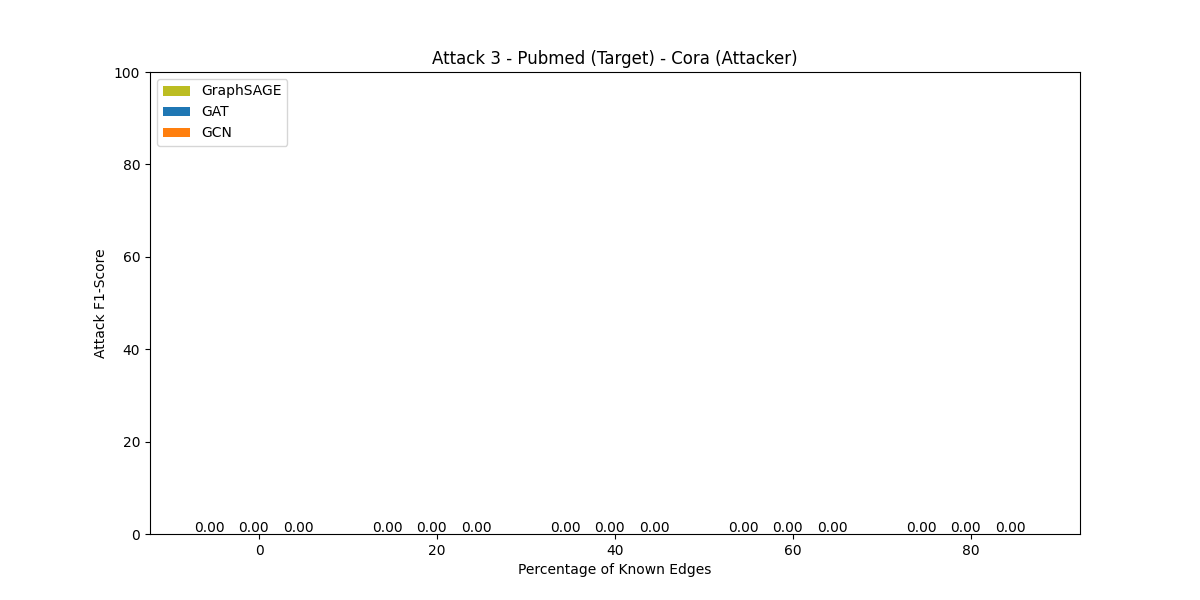
\includegraphics[width=\textwidth]{attack-3-pubmed-cora}
        \caption{Attack 3 - $D_{f_t} = Pubmed$ and $D_A = Cora$}
        \label{figure:eval-att3-cora-pubmed}
    \end{center}
  \end{figure}

  \begin{figure}[h]
      \begin{center}
          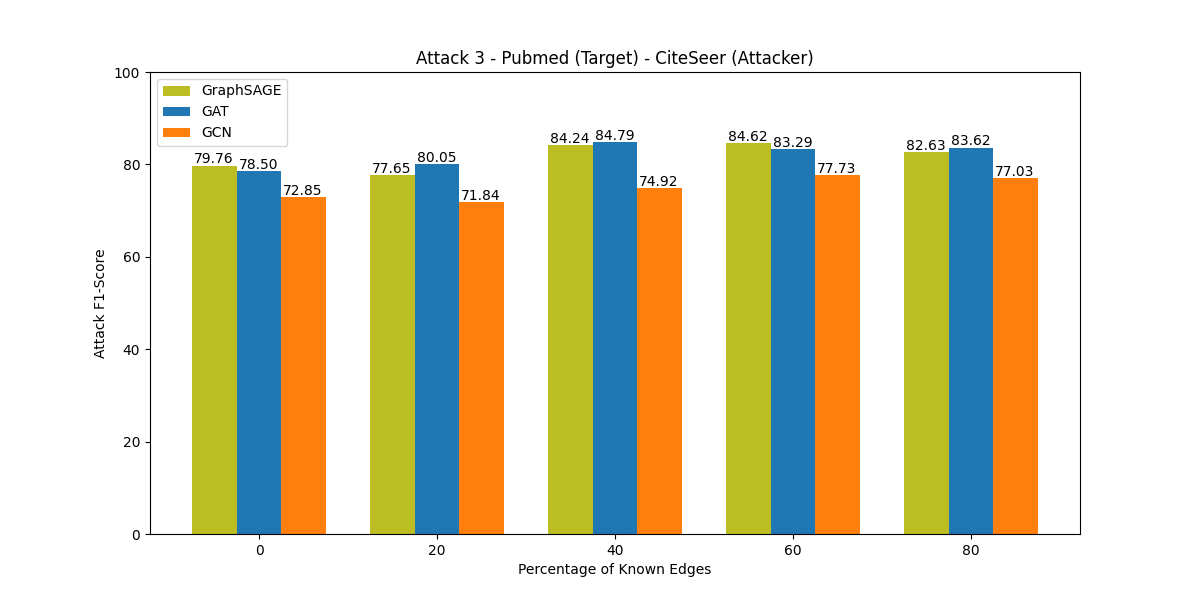
\includegraphics[width=\textwidth]{attack-3-pubmed-citeseer}
          \caption{Attack 3 - $D_{f_t} = Pubmed$ and $D_A = CiteSeer$}
          \label{figure:eval-att3-citeseer-pubmed}
      \end{center}
  \end{figure}